\documentclass{article}[11pt]

\usepackage{amsmath}
\usepackage{amssymb}
\usepackage{nicefrac}

\usepackage{pdflscape}

\usepackage{upgreek}

\usepackage{bashful}

% No intendation
\setlength\parindent{0pt}

\usepackage{hyperref}

\usepackage{siunitx}
\sisetup{
  per-mode=fraction,
  fraction-function=\tfrac
}

\usepackage{listings}
  \lstset{
    basicstyle=\ttfamily,
    escapeinside=||,
    xleftmargin=1cm
  }

\usepackage{float}

\usepackage{longtable}

\usepackage{multirow}

\usepackage{tikz}
  \usetikzlibrary{patterns}
  \usetikzlibrary{arrows.meta}
  \usetikzlibrary{shapes.misc}
  \usetikzlibrary{calc}

\usepackage{pgfplots}

\usepackage{cleveref}
\crefmultiformat{equation}{(#2#1#3)}{ and~(#2#1#3)}{, (#2#1#3)}{ and~(#2#1#3)}


\usepackage{acronym}
\usepackage[acronym,nonumberlist]{glossaries}
\glsdisablehyper
\makeglossaries
\newacronym{spice}{SPICE}{Simulation Program with Integrated Circuit Emphasis}
\newacronym{lef}{LEF}{Library Exchange Format}
\newacronym{dft}{DFT}{Discrete Fourier Transform}
\newacronym{dtft}{DTFT}{Discrete-Time Fourier Transform}
\newacronym{fft}{FFT}{Fast Fourier Transform}
\newacronym{mosfet}{MOSFET}{Metal–Oxide–Semiconductor Field-Effect Transistor}
\newacronym{clm}{CLM}{Channel Length Modulation}
\newacronym{de}{DE}{differential equation}
\newacronym{soi}{SOI}{silicon-on-insulator}
\newacronym{ldo}{LDO}{low-dropout regulator}
\newacronym{ota}{OTA}{operational-transconductance amplifier}
\newacronym{ofa}{OFA}{operational-floating amplifier}

% literature
\usepackage[ backend=biber
           , isbn=true
           , sorting=none
           , style=ieee
           ]{biblatex}
\addbibresource{./../../literature.bib}

% definitions
\def \whatis       {Notes}
\def \title        {Fuubar}

\def \author       {Matthias Schweikardt}

\def \authorMail   {mschweikardt@posteo.de}

\def \authorGithub {mschweikardt}

\def \license      {CC BY-SA 4.0}
\def \licenseUrl   {https://creativecommons.org/licenses/by-sa/4.0/}

\def \date         {nodate}

\def \pdfurl       {https://mschweikardt.github.io/ee-notes/%
\bash[stdout]
IFS=/ 
var=($PWD)
echo ${var[-1]}
\END%
.pdf
}
\def \srcurl       {srcurl}


% Customize footer and header of document
\usepackage{fancyhdr}

% Access last page number
\usepackage{lastpage}

% Access last page number
\usepackage[thinc]{esdiff}

% Physics
\usepackage{physics}

% Comment environment
\usepackage{comment}

% Subcaptions
\usepackage{subcaption}

% Thicker lines in tables
\usepackage{booktabs}

% Indentation in footnote
\makeatletter
\renewcommand\@makefntext[1]{\leftskip=2em\hskip-0.5em\@makefnmark#1}
\makeatother         

% qty with the siunitx definition
\AtBeginDocument{\RenewCommandCopy\qty\SI}

% TikZ compatibility
\pgfplotsset{compat=1.18}


\makeatletter
\pgfmathdeclarefunction{myatan2}{2}{%
\begingroup%
  \pgfmathfloattofixed{#1}\edef\tempa{\pgfmathresult}%
  \pgfmathfloattofixed{#2}%
  \pgfkeys{pgf/fpu=false}%
  \pgfmathparse{atan2(\tempa,\pgfmathresult)}\pgfkeys{/pgf/fpu}%
  \pgfmathfloatparsenumber{\pgfmathresult}%
  \pgfmath@smuggleone\pgfmathresult%
\endgroup
}
\makeatother

\usepackage{tabularx}
% usepackages
\usepackage[ a4paper
           , textwidth  = 16.0cm
           , textheight = 25.0cm
           , headsep    =  0.25cm
           , voffset    =  0.3cm
           , footskip   =  1.25cm
           ]{geometry}

% Section and subsection enumeration
\renewcommand{\thesection}{\Roman{section}.} 
\renewcommand{\thesubsection}{\thesection\Alph{subsection}}

\usepackage{titlesec}
\titleformat{\section}
  {\normalfont\Large\bfseries}{\thesection}{0.2em}{}
\titleformat{\subsection}
  {\normalfont\large\bfseries}{\thesubsection}{0.2em}{}


% Defince title of document
\newcommand{\notetitle}{
  \begingroup
  \hypersetup{hidelinks}
  \thispagestyle{notefirst}
  \begin{center}
  \rule{\textwidth}{1pt}\\
  \medskip
  {\it \whatis}\\
  \bigskip
  {\LARGE \textbf{\title}}\\
  \medskip
  {\small \author}\\
  \rule{\textwidth}{0.5pt}\\
  {\small
    \begin{minipage}[t]{0.5\textwidth}
      \begin{tabular}[t]{ p{2.25cm} p{5.75cm}}
        Mail: & \href{mailto:\authorMail}{\tt{\authorMail}} \\
        Github: & \href{https://github.com/\authorGithub}{\tt{\authorGithub}} \\
      \end{tabular}
    \end{minipage}%
    %
    \begin{minipage}[t]{0.5\textwidth}
      \begin{tabular}[t]{ p{2.25cm} p{5.75cm} }
        Date: & \date  \\
        License: & \href{\licenseUrl}{\license}
      \end{tabular}
    \end{minipage}
  }%
  {\small
    \begin{minipage}[t]{\textwidth}
      \begin{tabular}[t]{ p{2.25cm} p{12cm}}
        Latest PDF: & \href{\pdfurl}{\tt{\pdfurl}} \\
        Latest Source: & \href{\srcurl}{\tt{\srcurl}}
      \end{tabular}
    \end{minipage}%
  }
  \bigskip
  \rule{\textwidth}{1pt}
  \end{center}
  \endgroup
}

% Header and footer on first page
\fancypagestyle{notefirst}{
  \fancyhf{}
  \renewcommand{\headrulewidth}{0pt}
  \renewcommand{\footrulewidth}{0pt}

  \fancyfoot[C]{\thepage/\pageref*{LastPage}}
}

% Header and footer on 2nd-last page
\fancypagestyle{noterest}{
  \fancyhf{}
  \renewcommand{\headrulewidth}{0.5pt}
  \renewcommand{\footrulewidth}{0.0pt}

  \fancyhead[L]{\author}
  \fancyhead[C]{\title}
  \fancyhead[R]{\date}

  \fancyfoot[C]{\thepage/\pageref*{LastPage}}
}
\pagestyle{noterest}

\usepackage{amsmath}
\usepackage{amssymb}
\usepackage{nicefrac}

\usepackage{pdflscape}

\usepackage{upgreek}

\usepackage{bashful}

% No intendation
\setlength\parindent{0pt}

\usepackage{hyperref}

\usepackage{siunitx}
\sisetup{
  per-mode=fraction,
  fraction-function=\tfrac
}

\usepackage{listings}
  \lstset{
    basicstyle=\ttfamily,
    escapeinside=||,
    xleftmargin=1cm
  }

\usepackage{float}

\usepackage{longtable}

\usepackage{multirow}

\usepackage{tikz}
  \usetikzlibrary{patterns}
  \usetikzlibrary{arrows.meta}
  \usetikzlibrary{shapes.misc}
  \usetikzlibrary{calc}

\usepackage{pgfplots}

\usepackage{cleveref}
\crefmultiformat{equation}{(#2#1#3)}{ and~(#2#1#3)}{, (#2#1#3)}{ and~(#2#1#3)}


\usepackage{acronym}
\usepackage[acronym,nonumberlist]{glossaries}
\glsdisablehyper
\makeglossaries
\newacronym{spice}{SPICE}{Simulation Program with Integrated Circuit Emphasis}
\newacronym{lef}{LEF}{Library Exchange Format}
\newacronym{dft}{DFT}{Discrete Fourier Transform}
\newacronym{dtft}{DTFT}{Discrete-Time Fourier Transform}
\newacronym{fft}{FFT}{Fast Fourier Transform}
\newacronym{mosfet}{MOSFET}{Metal–Oxide–Semiconductor Field-Effect Transistor}
\newacronym{clm}{CLM}{Channel Length Modulation}
\newacronym{de}{DE}{differential equation}
\newacronym{soi}{SOI}{silicon-on-insulator}
\newacronym{ldo}{LDO}{low-dropout regulator}
\newacronym{ota}{OTA}{operational-transconductance amplifier}
\newacronym{ofa}{OFA}{operational-floating amplifier}

% literature
\usepackage[ backend=biber
           , isbn=true
           , sorting=none
           , style=ieee
           ]{biblatex}
\addbibresource{./../../literature.bib}

% definitions
\def \whatis       {Notes}
\def \title        {Fuubar}

\def \author       {Matthias Schweikardt}

\def \authorMail   {mschweikardt@posteo.de}

\def \authorGithub {mschweikardt}

\def \license      {CC BY-SA 4.0}
\def \licenseUrl   {https://creativecommons.org/licenses/by-sa/4.0/}

\def \date         {nodate}

\def \pdfurl       {https://mschweikardt.github.io/ee-notes/%
\bash[stdout]
IFS=/ 
var=($PWD)
echo ${var[-1]}
\END%
.pdf
}
\def \srcurl       {srcurl}


% Customize footer and header of document
\usepackage{fancyhdr}

% Access last page number
\usepackage{lastpage}

% Access last page number
\usepackage[thinc]{esdiff}

% Physics
\usepackage{physics}

% Comment environment
\usepackage{comment}

% Subcaptions
\usepackage{subcaption}

% Thicker lines in tables
\usepackage{booktabs}

% Indentation in footnote
\makeatletter
\renewcommand\@makefntext[1]{\leftskip=2em\hskip-0.5em\@makefnmark#1}
\makeatother         

% qty with the siunitx definition
\AtBeginDocument{\RenewCommandCopy\qty\SI}

% TikZ compatibility
\pgfplotsset{compat=1.18}


\makeatletter
\pgfmathdeclarefunction{myatan2}{2}{%
\begingroup%
  \pgfmathfloattofixed{#1}\edef\tempa{\pgfmathresult}%
  \pgfmathfloattofixed{#2}%
  \pgfkeys{pgf/fpu=false}%
  \pgfmathparse{atan2(\tempa,\pgfmathresult)}\pgfkeys{/pgf/fpu}%
  \pgfmathfloatparsenumber{\pgfmathresult}%
  \pgfmath@smuggleone\pgfmathresult%
\endgroup
}
\makeatother

\usepackage{tabularx}


\def \title  {Bode Plot}
\def \date   {September 19, 2025}

\def \pdfurl {https://mschweikardt.github.io/ee-notes/bode-plot.pdf}
\def \srcurl {https://github.com/mschweikardt/ee-notes/tree/main/notes/bode-plot}

\usepackage[scale=5]{draftwatermark}

\begin{document}

\notetitle

\section{Single Pole}

\begin{figure}[ht]
  \centering
  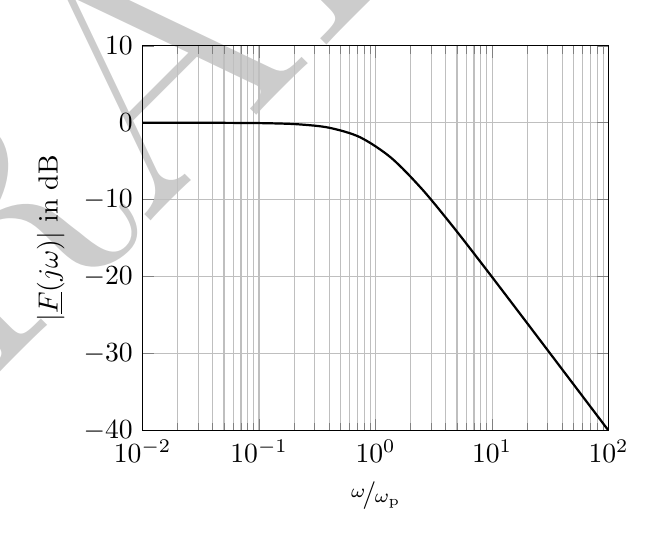
\begin{tikzpicture}
    \begin{axis}[ ylabel=$\left|\underline{F}(j\omega)\right|$ in \si{\decibel}
                , xlabel=$\nicefrac{\omega}{\omega_{\mathrm{p}}}$
                , xmode=log
                , ymin=-40
                , ymax=10
                , xmin=0.01
                , xmax=100
                , grid=both
                , width=7.5cm
                , ytick={-40,-30,...,10}
                ]
       \addplot[ domain=0.01:100
               , samples=16
               , smooth
               , thick] {-20*log10(sqrt(1+x^2))};
    \end{axis}
  \end{tikzpicture}
  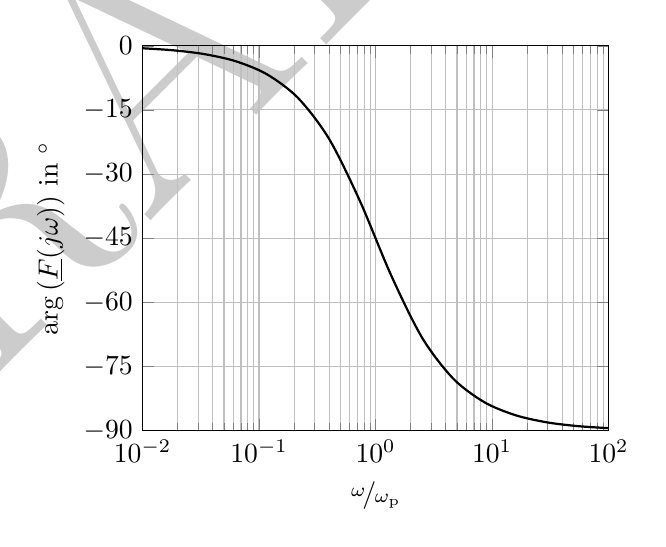
\begin{tikzpicture}
    \begin{axis}[ ylabel=$\arg\left(\underline{F}(j\omega)\right)$ in \si{\degree}
                , xlabel=$\nicefrac{\omega}{\omega_{\mathrm{p}}}$
                , xmode=log
                , ymin=-90
                , ymax=0
                , xmin=0.01
                , xmax=100
                , grid=both
                , width=7.5cm
                , ytick={-90,-75,...,0}
                ]

       \addplot[ domain=0.01:100
               , samples=16
               , smooth
               , thick] {-atan(x)};
    \end{axis}
  \end{tikzpicture}
  \caption{Bode plot of a single pole}
  \label{fig:bode:pole}
\end{figure}




\section{Single Zero}

\begin{figure}[ht]
  \centering
  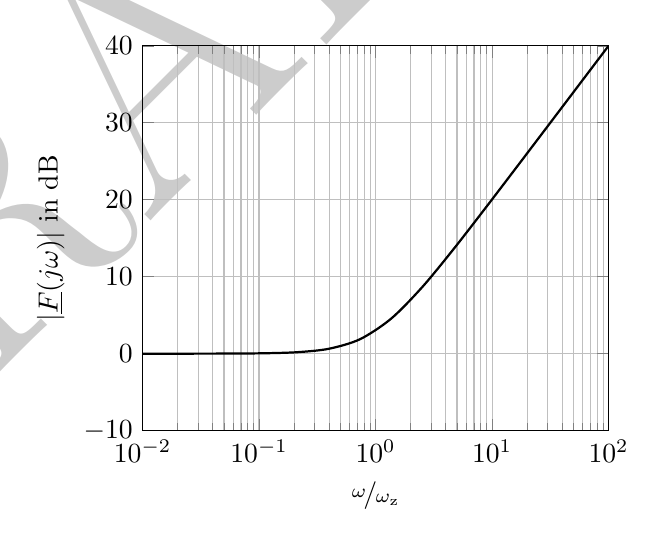
\begin{tikzpicture}
    \begin{axis}[ ylabel=$\left|\underline{F}(j\omega)\right|$ in \si{\decibel}
                , xlabel=$\nicefrac{\omega}{\omega_{\mathrm{z}}}$
                , xmode=log
                , ymin=-10
                , ymax=40
                , xmin=0.01
                , xmax=100
                , grid=both
                , width=7.5cm
                , ytick={-10,0,...,40}
                ]
       \addplot[ domain=0.01:100
               , samples=16
               , smooth
               , thick] {20*log10(sqrt(1+x^2))};
    \end{axis}
  \end{tikzpicture}
  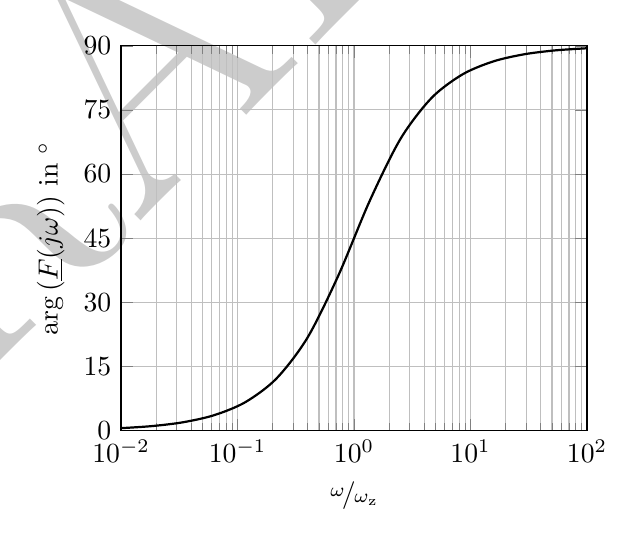
\begin{tikzpicture}
    \begin{axis}[ ylabel=$\arg\left(\underline{F}(j\omega)\right)$ in \si{\degree}
                , xlabel=$\nicefrac{\omega}{\omega_{\mathrm{z}}}$
                , xmode=log
                , ymin=0
                , ymax=90
                , xmin=0.01
                , xmax=100
                , grid=both
                , width=7.5cm
                , ytick={0,15,...,90}
                ]

       \addplot[ domain=0.01:100
               , samples=16
               , smooth
               , thick] {atan(x)};
    \end{axis}
  \end{tikzpicture}
  \caption{Bode plot of a single zero}
  \label{fig:bode:zero}
\end{figure}

\section{Zero-Pole Doublet}

\begin{equation}\label{eq:fs}
\underline{F}(j\omega) = \frac{1+\frac{j\omega}{\omega_{\mathrm{z}}}}{1+\frac{j\omega}{\omega_{\mathrm{p}}}}
\end{equation}

\begin{equation}
\omega_{\mathrm{p}} > \omega_{\mathrm{z}} > 0
\end{equation}

\begin{figure}[ht]
  \centering
  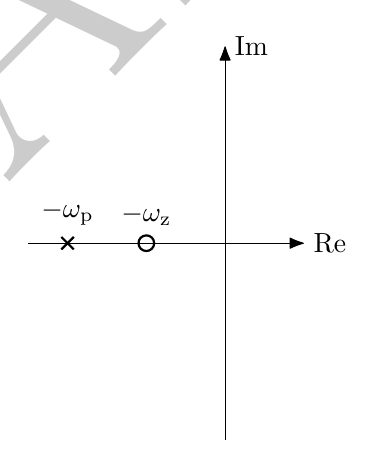
\begin{tikzpicture}[scale=1.0]
    \draw[-{Latex[round,scale=1.2,round]}] (-2.5,0) -- (1,0);
    \node[anchor=west] at (1,0) {Re};
    \draw[-{Latex[round,scale=1.2,round]}] (0,-2.5) -- (0,2.5);
    \node[anchor=west] at (0,2.5) {Im};

    \node[cross out,draw=black,thick,scale=0.6] at (-2, 0) {};
    \node[circle,draw=black,thick,scale=0.6] at (-1, 0) {};
    \node[anchor=south] at (-2, 0.1) {$-\omega_{\mathrm{p}}$};
    \node[anchor=south] at (-1, 0.1) {$-\omega_{\mathrm{z}}$};
  \end{tikzpicture}
  \caption{Pole-zero plot}
  \label{fig:pz-plot}
\end{figure}

\begin{equation}
\delta \stackrel{!}{=} \frac{\omega_{\mathrm{p}}}{\omega_{\mathrm{z}}}
\end{equation}

\begin{equation}
\left|\underline{F}(j\omega)\right|_{\mathrm{dB}} = 10 \cdot\log\left(1+\left(\frac{\omega}{\omega_{\mathrm{z}}}\right)^2\right)
                                                  - 10 \cdot\log\left(1+\left(\frac{1}{\delta} \frac{\omega}{\omega_{\mathrm{z}}}\right)^2\right)
\end{equation}

\begin{equation}
\begin{split}
\arg\left(\underline{F}(j\omega)\right) &= \arctan\left(\frac{\omega}{\omega_{\mathrm{z}}}\right) - \arctan\left(\frac{\omega}{\omega_{\mathrm{p}}}\right) \\
                                        &= \arctan\left(\frac{\omega}{\omega_{\mathrm{z}}}\right) - \arctan\left(\frac{1}{\delta} \frac{\omega}{\omega_{\mathrm{z}}}\right)
\end{split}
\end{equation}



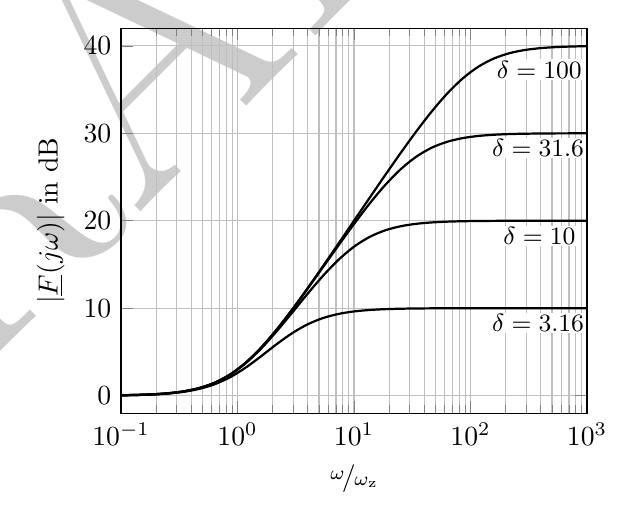
\begin{tikzpicture}
  \begin{axis}[ ylabel=$\left|\underline{F}(j\omega)\right|$ in \si{\decibel}
              , xlabel=$\nicefrac{\omega}{\omega_{\mathrm{z}}}$
              , xmode=log
              , ymin=-2
              , ymax=42
              , xmin=0.1
              , xmax=1000
              , grid=both
              , width=7.5cm
              ]

     \addplot[ domain=0.1:1000
             , samples=31
             , smooth
             , thick] {20*log10(sqrt(1+x^2))-20*log10(sqrt(1+(x/3.16225)^2))};             
     \addplot[ domain=0.1:1000
             , samples=31
             , smooth
             , thick] {20*log10(sqrt(1+x^2))-20*log10(sqrt(1+(x/10)^2))}; 
     \addplot[ domain=0.1:1000
             , samples=31
             , smooth
             , thick] {20*log10(sqrt(1+x^2))-20*log10(sqrt(1+(x/31.6225)^2))};
     \addplot[ domain=0.1:1000
             , samples=31
             , smooth
             , thick] {20*log10(sqrt(1+x^2))-20*log10(sqrt(1+(x/100)^2))}; 

      \node[anchor=north,font=\small,fill=white,inner sep=0.5pt] 
        at (axis cs:380,9.5) {$\delta=3.16$};
      \node[anchor=north,font=\small,fill=white,inner sep=0.5pt] 
        at (axis cs:390,19.5) {$\delta=10$};
      \node[anchor=north,font=\small,fill=white,inner sep=0.5pt] 
        at (axis cs:380,29.5) {$\delta=31.6$};
      \node[anchor=north,font=\small,fill=white,inner sep=0.5pt] 
        at (axis cs:390,38.5) {$\delta=100$};
  \end{axis}
\end{tikzpicture}
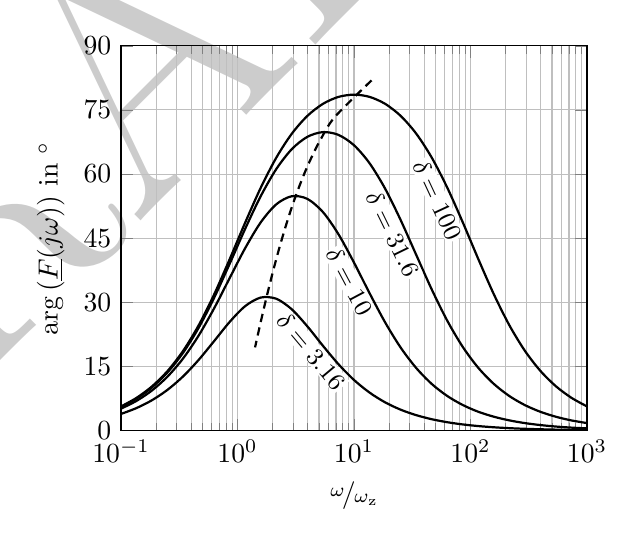
\begin{tikzpicture}
  \begin{axis}[ ylabel=$\arg\left(\underline{F}(j\omega)\right)$ in \si{\degree}
              , xlabel=$\nicefrac{\omega}{\omega_{\mathrm{z}}}$
              , xmode=log
              , ymin=0
              , ymax=90
              , xmin=0.1
              , xmax=1000
              , grid=both
              , width=7.5cm
              , ytick={0,15,...,90}
              ]

     \addplot[ domain=0.1:1000
             , samples=31
             , smooth
             , thick] {atan(x)-atan(x/3.16225)}; 
     \addplot[ domain=0.1:1000
             , samples=31
             , smooth
             , thick] {atan(x)-atan(x/10)}; 
     \addplot[ domain=0.1:1000
             , samples=31
             , smooth
             , thick] {atan(x)-atan(x/31.6225)}; 
     \addplot[ domain=0.1:1000
             , samples=31
             , smooth
             , thick] {atan(x)-atan(x/100)}; 

     \addplot[ domain=0.005:0.5
             , samples=31
             , smooth
             , densely dashed
             , thick] ({1/sqrt(x)},{atan(1/sqrt(x))-atan(sqrt(x))}); 

      \node[anchor=east,font=\small,fill=white,inner sep=0.5pt,rotate=-50] 
        at (axis cs:7.9,10) {$\delta=3.16$};
      \node[anchor=east,font=\small,fill=white,inner sep=0.5pt,rotate=-62] 
        at (axis cs:13,27) {$\delta=10$};
      \node[anchor=north,font=\small,fill=white,inner sep=0.5pt,rotate=-64] 
        at (axis cs:26,47) {$\delta=31.6$};
      \node[anchor=north,font=\small,fill=white,inner sep=0.5pt,rotate=-65] 
        at (axis cs:63,55) {$\delta=100$};
  \end{axis}
\end{tikzpicture}

Peak of phase (dashed line) at
\begin{equation}
\frac{\omega_{\mathrm{m}}}{\omega_{\mathrm{z}}} = \sqrt{\delta}
\end{equation}
with
\begin{equation}
\arg\left(\underline{F}(j\omega_{\mathrm{m}})\right) = 
  \arctan\left(\sqrt{\delta}\right)-\arctan\left(\frac{1}{\sqrt{\delta}}\right)
\end{equation}


\begin{figure}[ht]
  \centering
  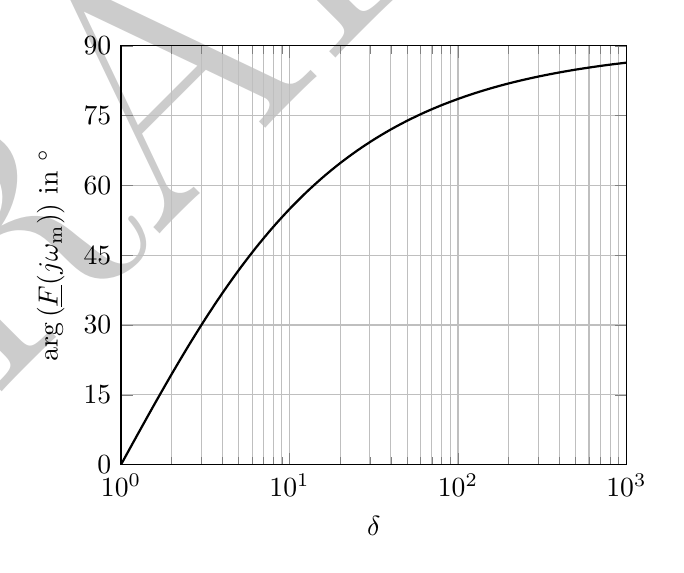
\begin{tikzpicture}
    \begin{axis}[ ylabel=$\arg\left(\underline{F}(j\omega_{\mathrm{m}})\right)$ in \si{\degree}
                , xlabel=$\delta$
                , xmode=log
                , ymin=0
                , ymax=90
                , xmin=1
                , xmax=1000
                , grid=both
                , width=8cm
                , ytick={0,15,...,90}
                ]

       \addplot[ domain=1:1000
               , samples=31
               , smooth
               , thick] {atan(sqrt(x))-atan(1/sqrt(x))}; 

    \end{axis}
  \end{tikzpicture}
  \caption{Maximum peak of phase boost}
  \label{fig:phase-boost}
\end{figure}



\printbibliography
\end{document}